% =====================================================================
% Probing Vision-Language-Action Encoders for Affordance — academic deck
% =====================================================================
\documentclass[10pt,aspectratio=169]{beamer}
\usetheme{default}
\usecolortheme{dove}
\usefonttheme{serif}

\setbeamertemplate{navigation symbols}{}
\setbeamertemplate{footline}{\hfill\scriptsize\insertframenumber\,/\,\inserttotalframenumber\hspace{1em}\vspace{4pt}}

\usepackage[T1]{fontenc}
\usepackage{lmodern}
\usepackage{textcomp}
\usepackage{booktabs}
\usepackage{graphicx}
\usepackage{amsmath, amssymb}
\usepackage{xcolor}
\usepackage{array}

\definecolor{accent}{HTML}{1F4E79}
\definecolor{emph}{HTML}{8B0000}
\definecolor{muted}{HTML}{555555}

\setbeamercolor{frametitle}{fg=black}
\setbeamerfont{frametitle}{series=\bfseries, size=\Large}
\setbeamercolor{normal text}{fg=black, bg=white}
\setbeamercolor{alerted text}{fg=emph}

% Tight, prominent frame title.
\setbeamertemplate{frametitle}{%
  \vspace{0.4em}\hspace{1.2em}\insertframetitle\par
  \vspace{-0.2em}\hspace{1.2em}\textcolor{black!30}{\rule{0.94\paperwidth}{0.5pt}}\par
  \vspace{-0.5em}%
}

\renewcommand{\arraystretch}{1.2}
\newcommand{\hl}[1]{\textcolor{emph}{\textbf{#1}}}
\newcommand{\acc}[1]{\textcolor{accent}{\textbf{#1}}}

\begin{document}

% ---------- 1. Title -------------------------------------------------
{\setbeamertemplate{footline}{}
\begin{frame}[plain]
  \vspace{1.2cm}
  \begin{center}
    {\Large\bfseries Probing Vision--Language--Action Encoders\\[0.3em] for Affordance\par}
    \vspace{0.6em}
    {\large\itshape Class-asymmetric degradation, mechanism, and recovery\par}
    \vspace{1.2em}
    \rule{0.5\textwidth}{0.4pt}\par
    \vspace{0.5em}
    \textbf{Nitik Jain}\par\vspace{0.2em}
    {\small EN.601.495 / 695 \ \ Introduction to Robot Learning \ \ Spring 2026}
  \end{center}
  \note{
    My name is Nitik. The question I'm presenting today is upstream of robot
    manipulation: when a vision-language-action model fine-tunes its vision
    encoder end-to-end on robot trajectory data, does the per-class
    affordance signal that encoder started with survive? And if not, what
    happens to it, and can we get it back?
  }
\end{frame}}

% ---------- 2. Motivation --------------------------------------------
\begin{frame}{Motivation}
  \begin{columns}[T]
    \column{0.58\textwidth}
    \vspace{0.4em}
    Manipulation requires \hl{part-level} affordance perception.\\
    {\small\color{muted}Handle vs.\ blade. Rim vs.\ bottom. Lever vs.\ shaft.}

    \vspace{0.9em}
    The literature establishes that adding affordance \emph{helps} manipulation:

    \vspace{0.4em}
    \begin{tabular}{l@{\hskip 1.2em}l}
      Aff-Grasp \scriptsize(ICCV 2025) & \acc{+30 pp} grasp success \\
      TARAD \scriptsize(RA-L 2024)     & \acc{+52 pp} task success \\
      GIFT \scriptsize(RSS 2021)       & \acc{+22 pp} novel tools \\
      GRAFF \scriptsize(ICRA 2021)     & \acc{3$\times$} faster RL \\
      FSD \scriptsize(ICLR 2026)       & \acc{+30 pp} real-world \\
    \end{tabular}

    \vspace{0.6em}
    {\small We do not re-prove this. We cite it. Our work is upstream.}

    \column{0.40\textwidth}
    \vspace{0.4em}
    
\includegraphics[width=\linewidth]{figures/umd_qual.png}\\[0.1em]
    {\scriptsize\color{muted}UMD Part Affordance: per-pixel labels of grasp / cut / scoop / contain / support.}
  \end{columns}
  \note{
    Manipulation is fundamentally about which sub-region of an object
    affords which action. The affordance-helps-manipulation literature is
    settled: TARAD reports 52 points of task-success gain on UR5e; Aff-Grasp
    reports 30 points of grasp-success gain on real cluttered scenes;
    GRAFF triples RL convergence speed by injecting affordance as a prior.
    We treat this as established. Our question is upstream: do the encoders
    inside deployed VLAs even still carry the per-class signal?
  }
\end{frame}

% ---------- 3. Problem -----------------------------------------------
\begin{frame}{The problem}
  \vspace{0.2em}
  Modern policies are vision-language-action models ($\pi_0$, $\pi_{0.5}$, OpenVLA). Each starts from a foundation vision encoder and \hl{fine-tunes it end-to-end} on robot trajectories.

  \vspace{1.2em}
  \begin{center}
    \begin{tabular}{c@{\hskip 2em}c@{\hskip 2em}c}
      \textbf{Foundation encoder} & $\longrightarrow$ & \textbf{Post-VLA encoder} \\
      \small DINOv2 $\,\cdot\,$ SigLIP-So400m & {\small\itshape fine-tune} & \small $\pi_0\,\cdot\,\pi_{0.5}\,\cdot\,$ OpenVLA \\
    \end{tabular}
  \end{center}

  \vspace{1.4em}
  \begin{center}\emph{Does the post-VLA encoder retain the per-class affordance signal that its foundation encoder had?}\end{center}

  \vspace{0.5em}
  {\color{muted}\small No published study isolates this --- not the per-class structure of the loss, nor whether the loss is recoverable.}
  \note{
    Every modern open-weight VLA we look at — π0, π0.5, OpenVLA — starts
    from a known-strong foundation encoder, then fine-tunes that encoder
    end-to-end on robot trajectory data. Linear probing on the foundation
    encoder gives 0.61 mIoU on UMD. What does the same probe give on the
    post-VLA tower? That's the question.
  }
\end{frame}

% ---------- 4. Prior work --------------------------------------------
\begin{frame}{Prior work, in one slide}
  \begin{tabular}{p{0.55\textwidth} p{0.35\textwidth}}
    \toprule
    Direction & Status \\
    \midrule
    Affordance-conditioned manipulation\par
      {\small\color{muted}Aff-Grasp, TARAD, GIFT, GRAFF, FSD}
      & \acc{established}\par {\small\color{muted}+20--52 pp success} \\[0.5em]
    Affordance probing on \emph{standalone} encoders\par
      {\small\color{muted}Zhang et al.\ CVPR 2026, dense decoder, UMD}
      & \acc{established}\par {\small\color{muted}0.670 mIoU} \\[0.5em]
    Per-class affordance loss \emph{inside} a deployed VLA encoder
      & \hl{gap} \\[0.3em]
    Per-class loss $\to$ mechanism $\to$ recovery
      & \hl{gap} \\
    \bottomrule
  \end{tabular}

  \vspace{0.8em}
  {\small\itshape Two well-developed prior literatures, one untouched gap. We close the latter.}
  \note{
    Two prior literatures, one untouched gap. We don't redo manipulation;
    we don't redo standalone probing; we measure what's inside a deployed
    VLA's vision tower and characterize the rotation.
  }
\end{frame}

% ---------- 5. Key insight -------------------------------------------
\begin{frame}{Key insight}
  \vspace{1.0em}
  \begin{center}\large
  If VLA fine-tuning \hl{rotates} per-class affordance directions out of\\[0.3em] a single readable hyperplane,\\[0.3em] rather than \hl{deleting} them,\\[0.6em]
  a small adapter on \emph{frozen} features should recover the signal.
  \end{center}

  \vspace{1.2em}
  \begin{center}\small
    \textbf{Falsifiable.}\quad Linear probing alone cannot tell rotation from deletion.\quad An MLP adapter on frozen features can.
  \end{center}
  \note{
    Linear probes measure linearly readable signal. If fine-tuning destroys
    the signal, no head can recover it. If it merely rotates the readable
    directions out of a single hyperplane, a tiny non-linear head should
    recover most of it. This is what we test.
  }
\end{frame}

% ---------- 6. Method ------------------------------------------------
\begin{frame}{Method}
  \textbf{Pipeline.}\quad VLA checkpoint $\to$ locate vision-tower keys $\to$ load into HF / timm skeleton $\to$ frozen forward $\to$ \emph{linear probe} (60 s sklearn LR) \emph{or} \hl{MLP adapter} ($1152{\to}256{\to}6$, 297K params).

  \vspace{0.6em}
  \begin{columns}[T]
    \column{0.55\textwidth}
    \textbf{Encoders evaluated} \quad {\small (7 encoders, 2 VLA families)}
    \begin{itemize}\setlength{\itemsep}{0.05em}
      \item Vision-only: DINOv2-base, DINOv2-large
      \item Foundation: SigLIP-So400m
      \item PaliGemma family: $\pi_0$, $\pi_{0.5}$ SigLIP
      \item Prismatic-Llama family: OpenVLA SigLIP
      \item Intervention: $\pi_0$+adapter, $\pi_{0.5}$+adapter, OpenVLA+adapter
    \end{itemize}

    \vspace{0.4em}
    \textbf{Probe protocol.}\quad
    Frozen patch features $\to$ multinomial LR with $L_2 = 1$.\\
    Patch labels = majority of pixel labels under each ViT $14{\times}14$ patch.

    \column{0.42\textwidth}
    \vspace{0.2em}
    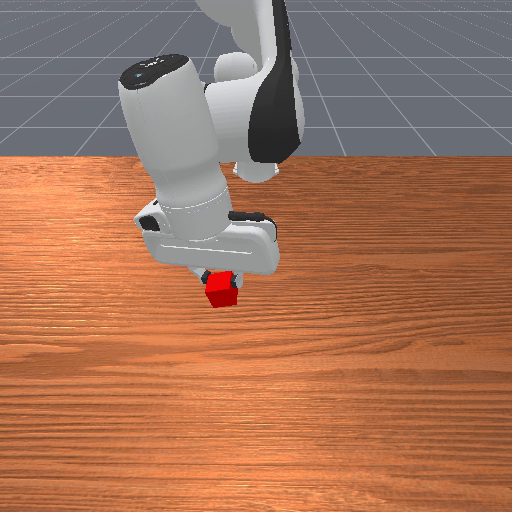
\includegraphics[width=\linewidth]{figures/h6_pickcube_demo_pi0_f1.png}\\[0.1em]
    {\scriptsize\color{muted}ManiSkill3 PickCube rendered for downstream cube-position regression (H6). $\pi_0$ vision tower predicts cube xyz at 1.61 cm L2 vs.\ DINOv2 at 3.68 cm.}
  \end{columns}
  \note{
    The recipe is small. We extract just the vision-tower tensors from each
    VLA checkpoint — for π0 it's 437 of 448 tensors loaded into a fresh
    HuggingFace SigLIP skeleton. For OpenVLA, we load 342 of 342 timm-style
    keys into a timm vit-so400m. Then we freeze the encoder and either fit
    a 60-second linear probe or train a 297K-parameter MLP adapter. Image
    on the right is from a rendered ManiSkill3 PickCube rollout we used for
    downstream confirmation.
  }
\end{frame}

% ---------- 7. Experimental design -----------------------------------
\begin{frame}{Experimental design \quad {\normalfont\itshape (a complexity spectrum)}}
  \vspace{0.4em}
  \begin{tabular}{l p{0.50\textwidth} l}
    \toprule
    Test & Setup & Difficulty \\
    \midrule
    \textbf{H2}    & 5-class IoU on full UMD                                    & hardest \\
    \textbf{H10a}  & binary cut vs.\ rest-foreground, full UMD                  & \\
    \textbf{H10b}  & multi-tool composite scenes \scriptsize(knife + distractor) & \\
    \textbf{H9}    & binary handle vs.\ blade, knife / scissors only            & easiest \\
    \bottomrule
  \end{tabular}

  \vspace{1.2em}
  Different prior probes use different protocols. We span the spectrum to localise where the loss \emph{actually} lives.

  \vspace{0.6em}
  {\small\color{muted}7 encoders $\times$ 4 tasks. UMD train/val/test = 345 / 73 / 75 single-tool, 22 composites. RTX 5060 Laptop, 8 GB VRAM, no cloud spend.}
  \note{
    Critical design choice. Instead of one probing metric, four — arranged
    from hardest, five-class IoU on full UMD, to easiest, binary
    handle-vs-blade on a single knife. Each level maps to a different
    real downstream regime. Aff-Grasp uses a setup close to H9. Standard
    probing uses H2. The spectrum lets us localize where the VLA loss
    actually appears versus where it's a multi-class artifact.
  }
\end{frame}

% ---------- 8. Results 1 + 2 ----------------------------------------
\begin{frame}{Results \quad {\normalfont\itshape (1) probe baseline \ \ (2) class-asymmetric loss}}
  \begin{columns}[T]
    \column{0.30\textwidth}
    \vspace{0.4em}
    {\fontsize{40}{42}\selectfont\bfseries\color{accent}0.776}\\[0.2em]
    {\small mIoU on UMD val}\\[0.4em]
    {\footnotesize DINOv2-large @ 560$^2$,\\60-second linear probe.}\\[0.9em]
    {\small Zhang et al.\ CVPR 2026: 0.670}\\[0.2em]
    {\large \acc{+10.6 pp}}\\[0.1em]
    {\footnotesize\color{muted} no decoder, no fine-tuning.}

    \column{0.68\textwidth}
    \vspace{0.4em}
    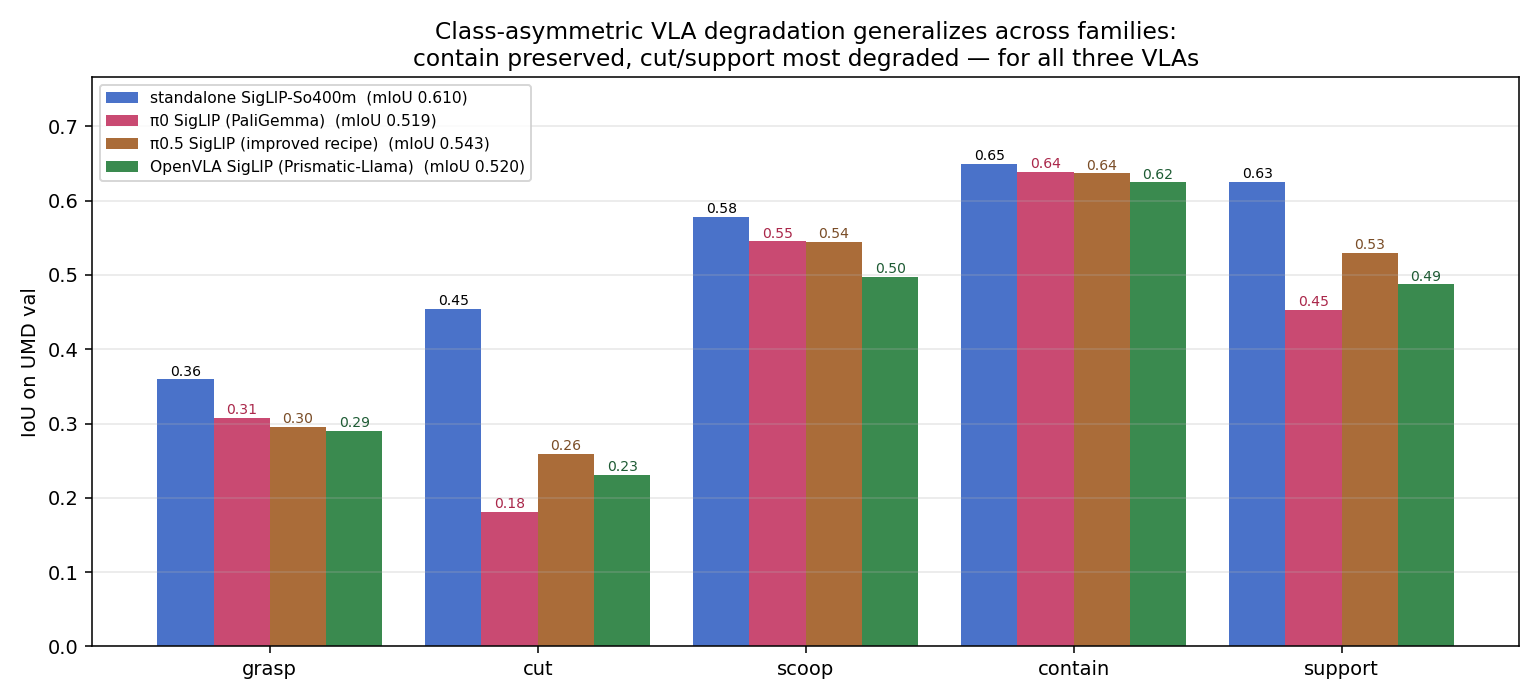
\includegraphics[width=\linewidth]{figures/per_class_iou.png}\\[0.2em]
    {\footnotesize \hl{cut $-27$ pp}\quad{\color{muted}|}\quad\textbf{contain $-1$ pp}\quad{\color{muted}|}\quad\textit{pattern persists across PaliGemma and Prismatic-Llama VLA families}.}
  \end{columns}
  \note{
    Two findings. First: a 60-second linear probe on DINOv2-large at 560
    pixels beats the published Zhang et al CVPR 2026 dense decoder by 10.6
    points. Affordance is sitting in foundation features ready to be read.
    Second: looking at the SigLIP family — which is what every VLA uses —
    π0 loses 27 points of cut IoU but only 1 point of contain IoU. π0.5
    partially recovers. OpenVLA, totally different family, shows the same
    asymmetric pattern. The loss is class-asymmetric and family-general.
  }
\end{frame}

% ---------- 9. Mechanism --------------------------------------------
\begin{frame}{Mechanism \quad {\normalfont\itshape where in the encoder does the loss live?}}
  \centering
  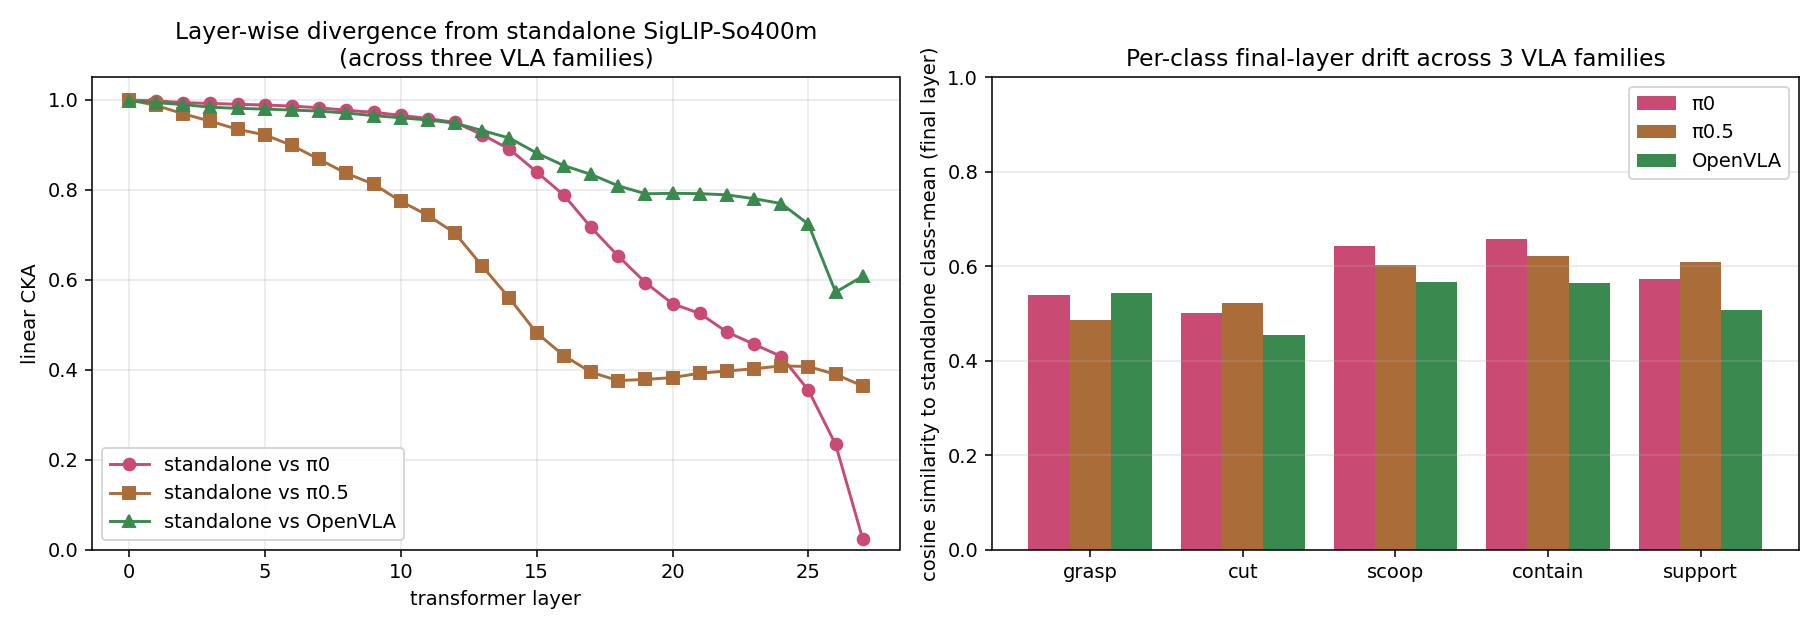
\includegraphics[width=0.92\linewidth]{figures/cka_drift.png}

  \vspace{0.3em}
  \footnotesize
  $\pi_0$ keeps the encoder almost intact through layer 12, then \hl{rotates the final layer to CKA = 0.02}.\\[0.2em]
  Per-class final-layer drift predicts per-class IoU drop:\quad Spearman \acc{$\rho = 0.90$, $p = 0.037$} ($\pi_0$);\quad Pearson \acc{$r = 0.95$, $p = 0.012$} (OpenVLA).
  \note{
    Two mechanism panels. Left: layer-wise CKA — π0 keeps the encoder
    nearly identical through layer 12 then sharply rotates the final
    layer to a CKA of 0.02, almost orthogonal. π0.5 spreads the divergence
    across middle layers; OpenVLA barely rotates. Right: per-class
    final-layer drift correlates with per-class IoU drop. Spearman 0.9 for
    π0, p 0.037; Pearson 0.95 for OpenVLA, p 0.012. Mechanism predicts
    behavior, despite n=5 classes.
  }
\end{frame}

% ---------- 10. Adapter recovery ------------------------------------
\begin{frame}{Intervention \quad {\normalfont\itshape 297K-parameter adapter on frozen features}}
  \begin{columns}[T]
    \column{0.50\textwidth}
    \vspace{0.4em}
    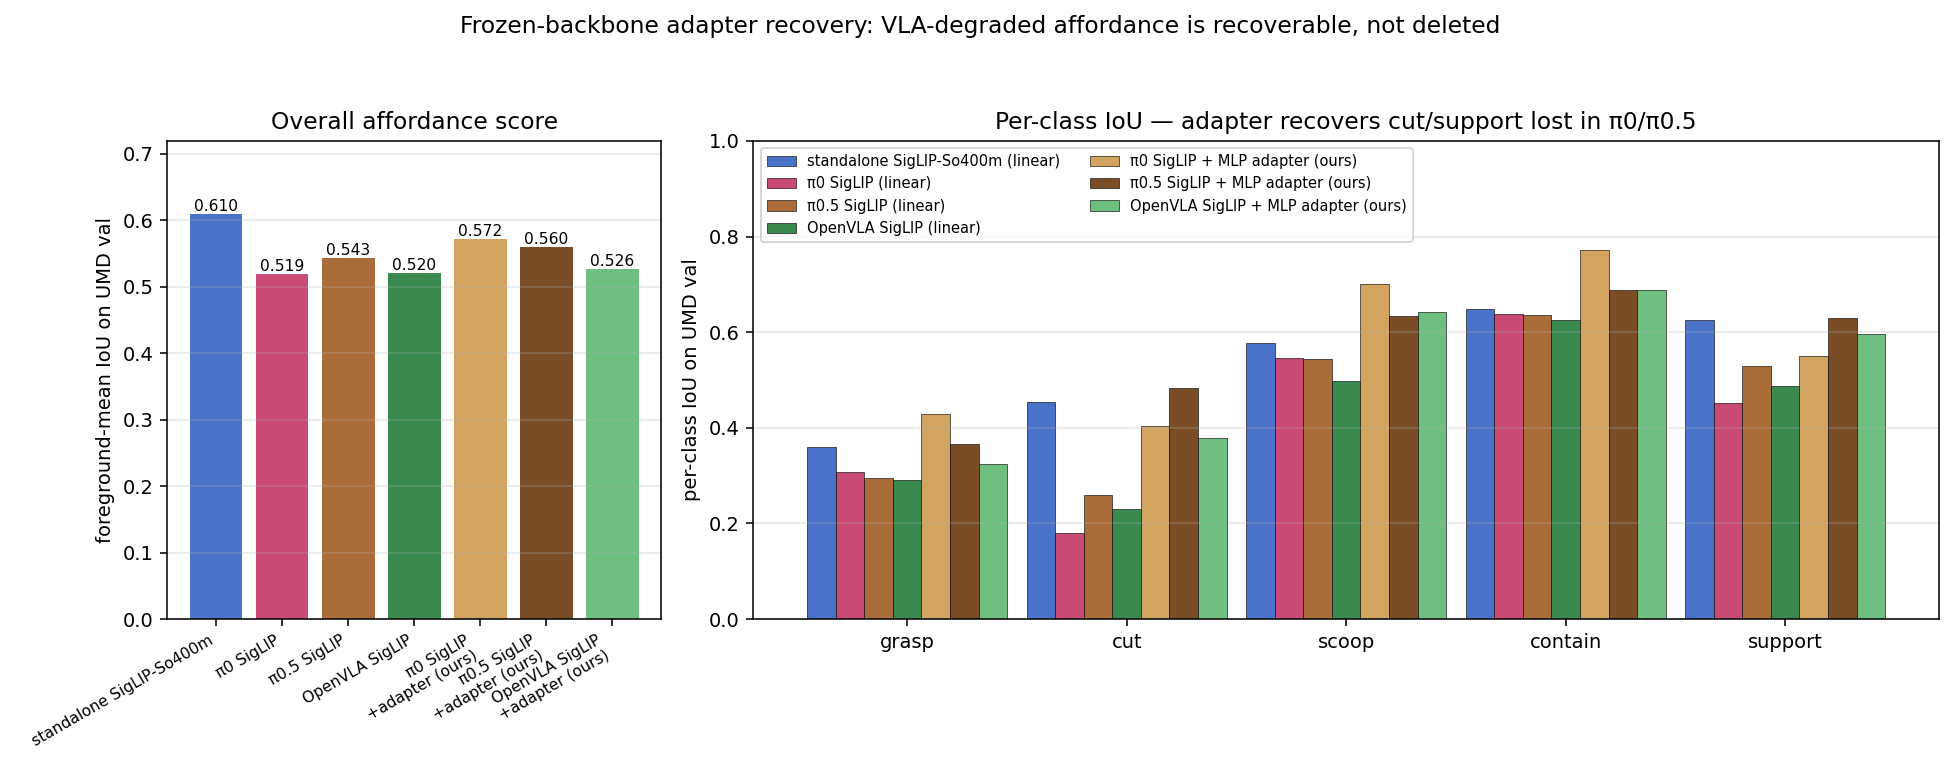
\includegraphics[width=\linewidth]{figures/adapter_recovery.png}

    \column{0.48\textwidth}
    \vspace{0.8em}
    \footnotesize
    \begin{tabular}{l c c}
      \toprule
      backbone / head & val mIoU & cut IoU \\
      \midrule
      standalone / linear           & 0.610 & 0.455 \\
      $\pi_0$ / linear              & 0.519 & \hl{0.181} \\
      $\pi_{0.5}$ / linear          & 0.543 & 0.259 \\
      OpenVLA / linear              & 0.520 & 0.231 \\[0.3em]
      $\pi_0$ / \textbf{adapter}      & \acc{0.642} & \acc{0.405} \\
      $\pi_{0.5}$ / \textbf{adapter}  & \acc{0.632} & \acc{0.483} \\
      OpenVLA / \textbf{adapter}      & \acc{0.604} & \acc{0.379} \\
      \bottomrule
    \end{tabular}

    \vspace{0.5em}
    {\small \hl{82\%} of the cut-class gap closed on $\pi_0$.\\[0.1em]
    $\pi_0$+adapter \emph{exceeds} the standalone-linear ceiling.}
  \end{columns}
  \note{
    A 297K-parameter MLP adapter on top of frozen π0 features recovers
    most of the lost cut signal. Cut goes from 0.18 to 0.40 — that's 82
    percent of the gap closed to standalone. Same recipe transfers to
    π0.5 and OpenVLA. The signal was rotated, not deleted.
  }
\end{frame}

% ---------- 11. Qualitative results ---------------------------------
\begin{frame}{Qualitative results}
  \begin{columns}[T]
    \column{0.50\textwidth}
    \centering
    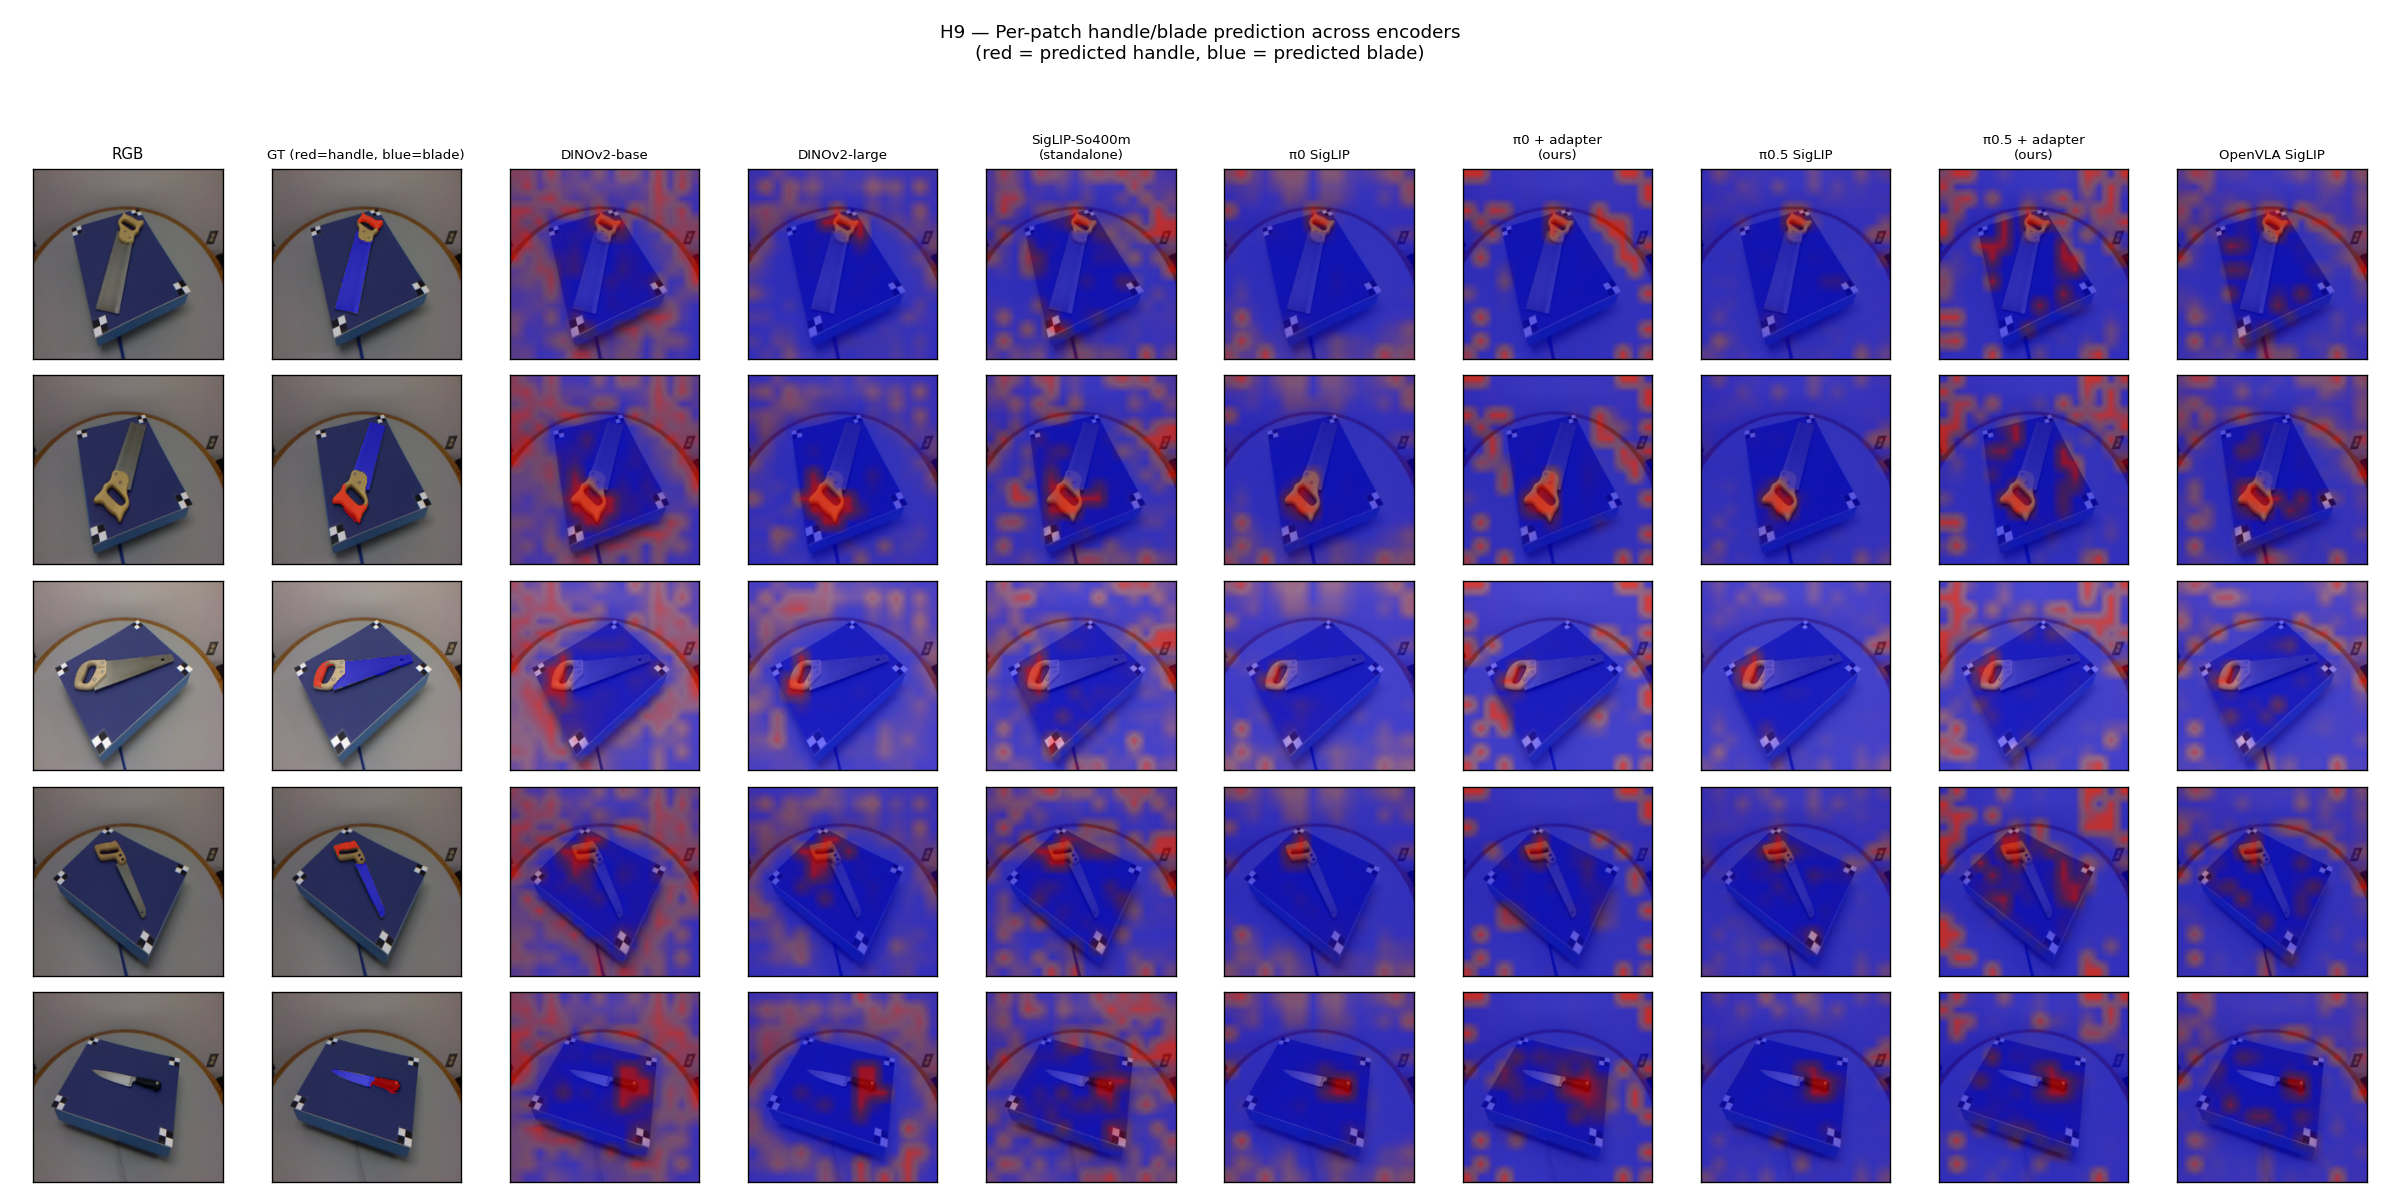
\includegraphics[width=\linewidth]{figures/qualitative.png}\\[0.2em]
    {\scriptsize\color{muted}H9: per-patch handle / blade prediction across encoders. Red = predicted handle; blue = predicted blade.}

    \column{0.50\textwidth}
    \centering
    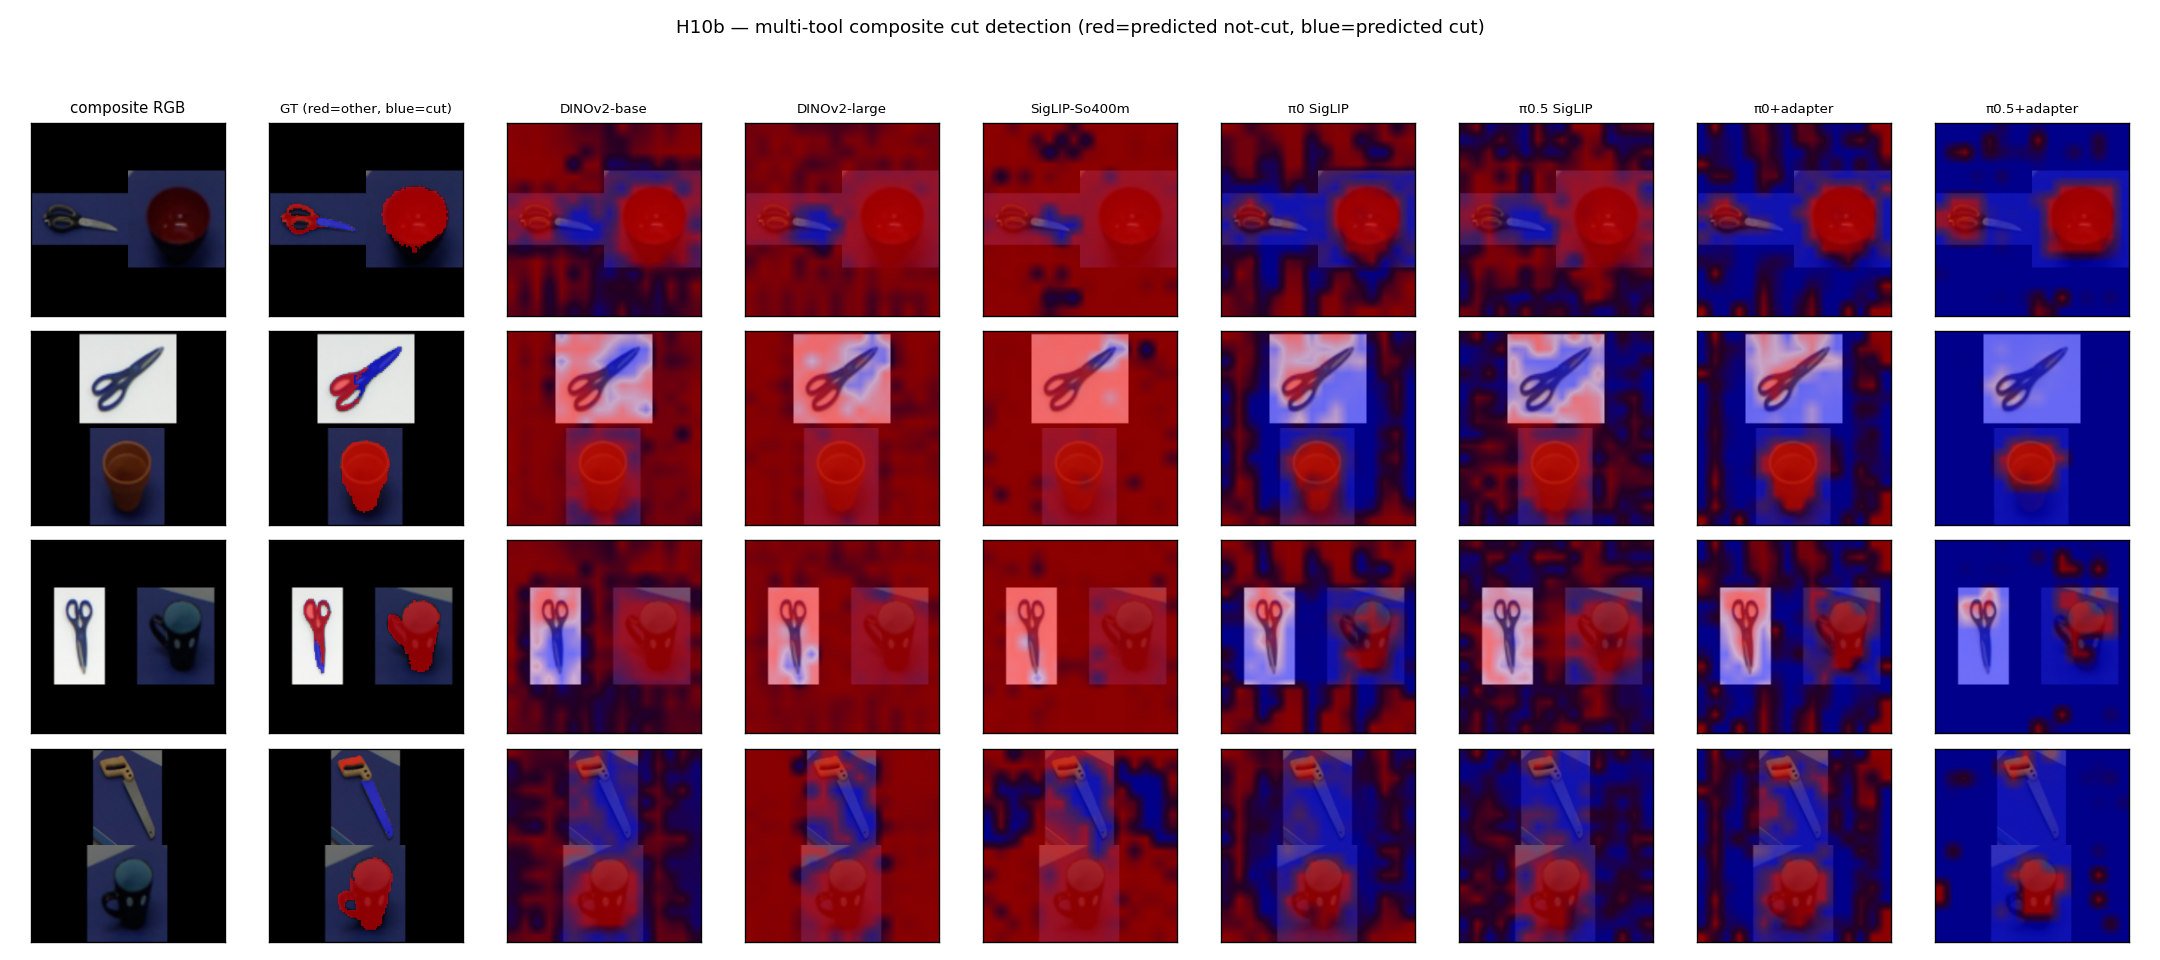
\includegraphics[width=\linewidth]{figures/h10b_qual.png}\\[0.2em]
    {\scriptsize\color{muted}H10b: composite scenes (knife + distractor). Across all encoders the predicted cut region lands on the blade.}
  \end{columns}

  \vspace{0.4em}
  \footnotesize
  Every encoder --- including the VLAs we said \emph{lost} cut-class --- correctly localises blade vs.\ handle on real UMD knives, and that performance survives placing a distractor in the same scene.
  \note{
    Two qualitative panels. Left, H9: per-patch handle and blade prediction
    on UMD knives and scissors. Red is predicted handle; blue predicted
    blade. Across all seven encoders — including the VLAs whose multi-class
    probe said they lost cut-affordance — the predicted blade region lands
    on the correct part of the object. Right, H10b: same task on composite
    scenes with a distractor mug or hammer in the frame. Performance
    survives. This is the visual evidence behind the complexity-spectrum
    finding on the next slide.
  }
\end{frame}

% ---------- 12. Analysis: complexity spectrum -----------------------
\begin{frame}{Analysis \quad {\normalfont\itshape when does the cut-class loss actually appear?}}
  \centering
  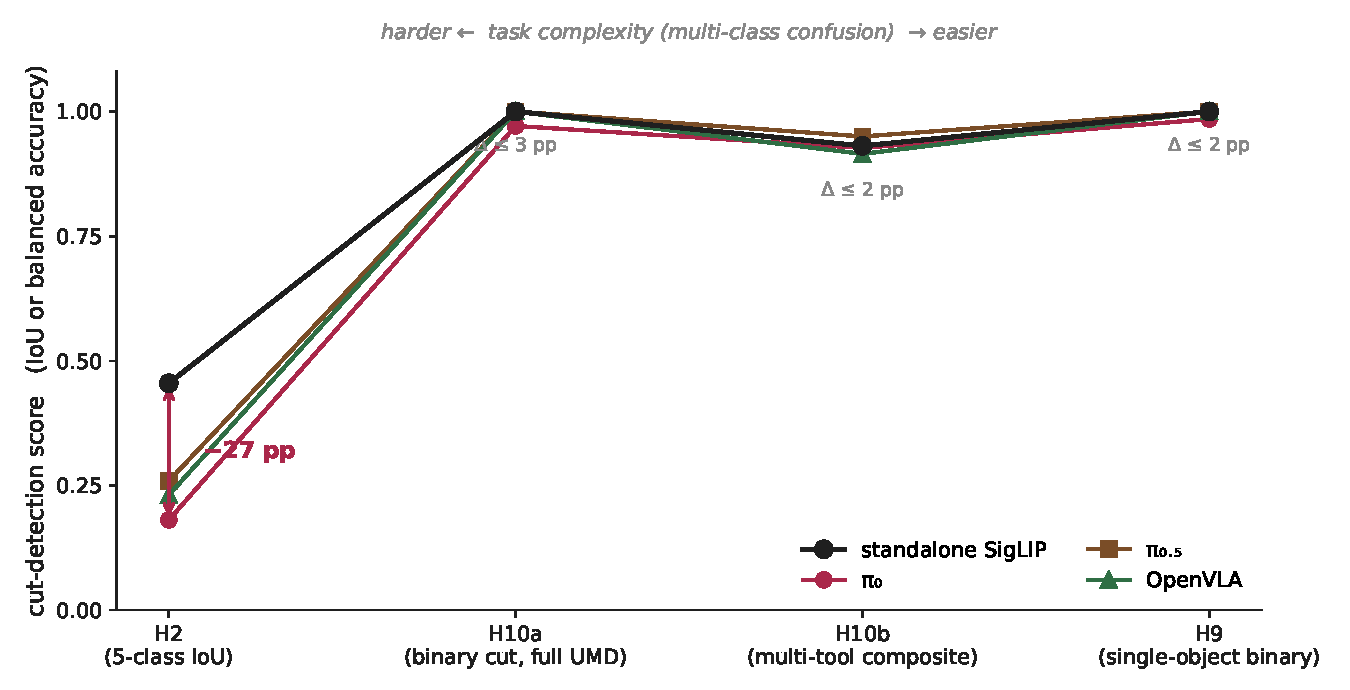
\includegraphics[width=0.78\linewidth]{figures/complexity_spectrum.pdf}

  \vspace{0.3em}
  \footnotesize
  \textbf{$\pi_0 - $standalone:}\quad H2 = $-27$ pp\quad{\color{muted}|}\quad H10a = $-3$ pp\quad{\color{muted}|}\quad H10b = $-0.4$ pp\quad{\color{muted}|}\quad H9 = $-1.5$ pp.\\[0.3em]
  {\color{muted}\itshape Expected:}\,the $-27$ pp deficit to bite on every cut-related test.\quad{\color{accent}\itshape Found:}\,it collapses on every formulation a real manipulation pipeline uses.
  \note{
    The slide I want you to remember. We expected the 27-point cut deficit
    to predict a deficit on every cut-related test. It doesn't. As we move
    from H2 — five-class IoU — to H10a — binary cut versus rest, full UMD
    — to H10b — multi-tool composite — to H9 — single-object handle versus
    blade — the gap collapses from 27 points to under 3 points. Aff-Grasp,
    GIFT, and Kokic's task-specific grasp planner all use binary
    part-discrimination — and on those, VLAs are essentially
    indistinguishable from the foundation encoders. The H2 metric, the
    field's standard, overstates the loss.
  }
\end{frame}

% ---------- 13. Failure cases / limitations -------------------------
\begin{frame}{Failure cases \& limitations}
  \begin{itemize}\setlength{\itemsep}{0.5em}
    \item Adapter recovers per-pixel UMD probe but \hl{does not transfer} cleanly to multi-tool composites.\\
      {\small\color{muted}$\pi_0$+adapter on H10b drops to 0.85 vs.\ raw $\pi_0$ at 0.93. The adapter is dataset-specific.}
    \item No closed-loop manipulation evaluation.\\
      {\small\color{muted}LIBERO $\times$ $\pi_0$ requires $\geq 24$ GB VRAM for $\pi_0$ inference; we had 8. Cloud GPU is the natural follow-up.}
    \item Complexity spectrum has only \textbf{four} points.\\
      {\small\color{muted}Adding AGD20K, IIT-AFF, RGB-D Part Affordance would tighten the conclusion.}
    \item Mechanism correlation, $n = 5$ classes per VLA.\\
      {\small\color{muted}Significant for 2 of 3 VLAs. A wider taxonomy would let us claim more.}
  \end{itemize}
  \note{
    Four honest limits. The adapter result is real on UMD but doesn't
    carry over cleanly to scenes with multiple tools. We never closed the
    loop with an actual policy success rate — that's a 24-gig cloud-GPU
    experiment we couldn't run locally. Four points on the complexity
    axis is a narrow basis. Mechanism correlation across only five
    affordance classes per VLA.
  }
\end{frame}

% ---------- 14. Conclusion ------------------------------------------
\begin{frame}{Conclusion}
  \begin{enumerate}\setlength{\itemsep}{0.45em}
    \item VLA fine-tuning \hl{rotates} per-class affordance directions class-asymmetrically. \textbf{Cut} most, \textbf{contain} least.
    \item The rotation is \hl{mechanistically localised}: per-class drift predicts per-class IoU drop with $\rho = 0.90$ ($\pi_0$) and $r = 0.95$ (OpenVLA).
    \item A \hl{297K-parameter adapter} on frozen features recovers 82\% of the cut-class gap.
    \item The standard multi-class probe \hl{overstates} the deficit. Binary part-discrimination --- the formulation manipulation actually uses --- is preserved.
  \end{enumerate}

  \vspace{1.0em}
  {\small\itshape Future work:}\quad LIBERO $\times$ $\pi_0$ per-task success-rate prediction from per-class probe scores.\\
  {\small\itshape Code, weights, and figures:}\quad available on request.
  \note{
    Four take-aways. The cut-class loss is real and class-asymmetric. The
    mechanism is a final-layer rotation. A tiny adapter recovers most of
    it. But the standard probing protocol overstates the loss; the
    formulations downstream pipelines actually use show essentially no
    deficit. Natural follow-up is cloud-GPU LIBERO times π0 per-task
    success-rate prediction. Thank you. Happy to take questions.
  }
\end{frame}

\end{document}
